\documentclass{article}
\usepackage[utf8]{inputenc}
\usepackage{amsmath,amsfonts,amssymb,amsthm}
\usepackage{bm}
\usepackage{booktabs}
\usepackage{caption}
\usepackage{commath}
\usepackage[hidelinks]{hyperref}
\usepackage{indentfirst}
\usepackage{natbib}
\usepackage{pgfplots}
\usepackage{subcaption}
\usepackage{tkz-euclide}

\title{Linear Algebra and the Primal Support Vector Machine}
\author{Matthew A. Nazari}
\date{December 2020}

\newtheorem{theorem}{Theorem}[section]
\newtheorem*{lemma}{Lemma}
\newtheorem{proposition}{Proposition}[section]

\theoremstyle{remark}
\newtheorem*{remark}{Remark}

\theoremstyle{definition}
\newtheorem{definition}{Definition}[section]

\hypersetup{
    colorlinks=true,
    linkcolor=black,
    urlcolor=blue,
    citecolor=black
}

\begin{document}
\maketitle

\tableofcontents

\newpage
\section{Cover Letter}

\vspace*{2cm}

\noindent To this paper's editors,

\vspace*{1.5cm}

The original intent of this paper was to provide a comprehensive introduction to a intermediate computer scientist like myself into the field of machine learning and explore the Support Vector Machine as an example. With the advice of Tarun and Dusty I realized this would entail an egregious amount of pages of mostly non-mathematical discussion on the principles behind general machine learning practices and concepts. As evident in my paper's length, I still prioritized offering a thorough and slow introduction to machine learning over brevity. However, the derivation of my paper ends with the primal form of the SVM which is an ideal balance between what this project expected of me and my original intentions. Almost the entirely of my original paper was scraped after the rough draft and by doing so I have achieved a paper which I am proud of.

The paper begins with an introduction for the motivation of an algorithm like the SVM in the machine learning setting. With concepts of linear algebra introduced between the lectures and the problem sets I develop various forms of the primal SVM. By viewing the primal SVM from multiple perspectives (hard margin, soft margin, regularization, etc.), I build intuition for not just the SVM as an algorithm but for the rationale behind modelling decisions and derivations in machine learning I wish I had at the beginning of this project. In this way, I am very proud to have preserved my original intention while fulfilling the expectations of the project.

\vspace*{1.5cm}

\noindent Sincerely,

\noindent Matthew A. Nazari

\newpage
\section{The Primal Support Vector Machine}

\subsection{An Introduction}

It is common for us to employ a machine learning algorithm to predict one of many discrete outcomes. A video streaming platform, for example, in order to abide by FTC guidelines might age-restrict videos they deem inappropriate for younger or more sensitive users. Consequently, this company might want an algorithm to predict whether a video is either ``mature" or ``family friendly". When there are only two discrete outcomes (``classes"), as in this example, the machine learning task is called binary classification. In this paper we will derive a fantastically competent algorithm called the support vector machine (SVM) designed to perform this exceedingly common machine learning task.

\subsubsection{Data Representation in Machine Learning}

\begin{figure}
    \centering
    \begin{subfigure}{0.49\textwidth}
        \centering
        \begin{tabular}{llll}\toprule
        Name   & Age  & Weight  & Height \\ \midrule
        Juan   & $18$ & $162$lb & $6$ft $1$in \\
        Joe    & $34$ & $146$lb & $5$ft $10$in \\
        Mei    & $39$ & $193$lb & $5$ft $8$in \\
        Bella  & $21$ & $124$lb & $5$ft $3$in \\
        Abdul  & $57$ & $141$lb & $5$ft $7$in \\
        Hanna  & $40$ & $134$lb & $5$ft $4$in \\ \bottomrule
        \end{tabular}
        \captionsetup{labelfont={bf}, textfont=it}
        \caption{Data in raw representation.}
        \label{fig:data represented by vectors a}
    \end{subfigure}
    \begin{subfigure}{0.5\textwidth}
        \centering
        \begin{tabular}{llll}\toprule
        Age  & Weight (kg) & Height (cm) \\ \midrule
        $18$ & $73.48$ & $185.42$ \\
        $34$ & $66.22$ & $177.80$ \\
        $39$ & $87.54$ & $172.72$ \\
        $21$ & $56.25$ & $160.02$ \\
        $57$ & $63.96$ & $170.18$ \\
        $40$ & $60.78$ & $162.56$ \\ \bottomrule
        \end{tabular}
        \captionsetup{labelfont={bf}, textfont=it}
        \caption{Data in numerical representation.}
        \label{fig:data represented by vectors b}
    \end{subfigure}    \captionsetup{labelfont={bf}, textfont=it, width=.8\linewidth}
    \caption{Data representations; raw data must be given a chosen numerical representations in order to be operated on by an algorithm.}
    \label{fig:data represented by vectors}
\end{figure}

The idea behind any machine learning algorithm is to reveal patterns and extrapolate information from data\footnote{For the scope of this paper we have omitted discussion of basic machine learning vocabulary; all concepts and terminology can be explored further in the \textit{Mathematics for Machine Learning} \citep{deisenroth2020mathematics}.}. Consider the example data set in Figure \ref{fig:data represented by vectors a}. like much of real world data sets each data point or ``example" (represented by rows) have non-numerical properties or ``features" (represented by columns). Hence, a programmer must chose a numerical representation for the data. With the aid of a domain expert, a chosen numerical representation might look like Figure \ref{fig:data represented by vectors b}. Some features like the individual's name may be left out not only for privacy but because that information probably does not lend insight on the task at hand. In this paper, and in machine learning convention, we denote the number of examples in a data set with $N$ and the number of features in each example with $D$. Therefore we can represent any example in a given data set as the vector $\bm{x}_n \in \mathbb{R}^D$:
\begin{definition}[Example vector]
    Given a data set of $N$ data points with $D$ features, the example vector $\bm{x}_n \in \mathbb{R}^D$ is the vector representation of the $n$-th data point in the data set, i.e., the $d$-th entry $\bm{x}_n^{(d)}$ of $\bm{x}_n$ is the $d$-th feature.
\end{definition}

With data representation understood we can now use concepts in linear algebra to extract information from the data. For example, measuring the distance between two example vectors is an empirical measurement of the similarity between those individuals.

\subsubsection{The SVM as an Algorithm}

Recall the task performed by the SVM is binary classification: therefore when presented an example the SVM must predict a class. The two binary classes are referred to as the ``positive class" and ``negative class" and expressed with the labels $+1$ and $-1$ respectively. A SVM that, for example, predicts diabetes in patients will output the label $+1$ for a positive diagnosis (positive class) and the label $-1$ for a negative diagnosis (negative class). This is done with the a predictor function: \begin{definition}[SVM predictor]
    An SVM predictor takes the form of a function which classifies an example $\bm{x} \in \mathbb{R}^D$ with the label $+1$ or negative $-1$ corresponding to either the positive or negative binary classes respectively:
    \begin{equation}
        f:\mathbb{R}^D \rightarrow \{+1,-1\}.
    \end{equation}
\end{definition}

The predictor function in any machine learning algorithm is a function employed by the algorithm's ``model" to perform the task at hand. The model is a mathematical construction that often only differs subtly from the predictor function. In a linear regression \citep{lay2016linear} setting, the model of the algorithm is a continuous function calculated by fitting certain ``model parameters" to a training data set with linear regression. By taking the machine learning approach we know our SVM algorithm will also have model parameters we will need to optimize on a training data set. The process of optimizing our model with training data is referred to as training or ``learning" a model.

As in any machine learning task, we would like to estimate parameters of our model given a training data set that minimizes classification error: recalling our previous example, mistakenly classifying a violent or pornographic video as family friendly is an error in the streaming platform's SVM algorithm the company would ideally minimize. The amount of error an algorithm incurs on unseen data like this is called ``variance" which is minimized by finding optimal parameters to our model that will fit unseen data accurately. Recalling our familiarity with linear regression, we are also minimizing variance by finding a line of best fit by deriving that line from a given training data set. In a linear regression situation, the model of the algorithm is a continuous function and we train the model by performing linear regression to find the best fit. In a similar way we must train our SVM model which we will see takes the form of solving an optimization problem on our training data. Before we derive what this optimization problem looks like, we must design our model.

\subsection{The SVM Model}

\subsubsection{The Hyperplane}

\begin{figure}
    \begin{center}
        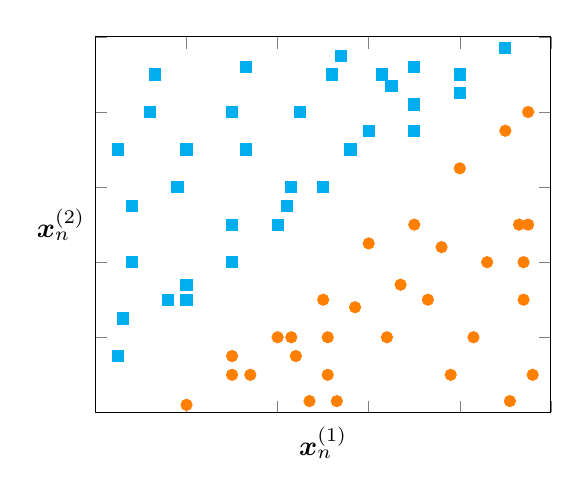
\begin{tikzpicture}
            \begin{axis}[ 
                width= 2.9in,
                height= 2.5in,
                xlabel=$\bm{x}_n^{(1)}$,
                ylabel={$\bm{x}_n^{(2)}$},
                yticklabels={,,},
                xticklabels={,,},
                xmin=0,
                xmax=10,
                ymin=0,
                ymax=10,
                every axis x label/.style={
                    at={(axis description cs:0.5,-0.15)},
                    anchor=south
                },
                every axis y label/.style={
                    at={(axis description cs:-0.15,.5)},
                    anchor=west
                },
            ]
            \addplot+[only marks,mark=square*,mark options={scale=1, color=cyan}] coordinates {
                (0.5,1.5) (0.6,2.5) (0.8,5.5) (0.8,4) (0.5,7)
                (1.2,8) (1.3,9) (1.6,3) (1.8,6) 
                (2,3) (2,3.4) (2,7) 
                (3,4) (3,8) (3,5) (3.3,7) (3.3,9.2)
                (4,5) (4.2,5.5) (4.3,6) (4.5,8) 
                (5,6) (5.2,9) (5.4,9.5) (5.6,7) 
                (6,7.5) (6.3,9) (6.5,8.7) 
                (7,7.5) (7,9.2) (7,8.2) 
                (8,8.5) (8,9)
                (9,9.7)
            };
            
            \addplot+[only marks,mark=*,mark options={scale=1, color=orange}] coordinates {
                (2,0.2)
                (3,1.5) (3,1) (3.4,1) 
                (4,2) (4.7,0.3) (4.4,1.5) (4.3,2) 
                (5,3) (5.1,1) (5.1,2) (5.3,0.3) (5.7,2.8) 
                (6,4.5) (6.4,2) (6.7,3.4) 
                (7,5) (7.3,3) (7.8,1) (7.6,4.4) 
                (8,6.5) (8.3,2) (8.6,4) 
                (9,7.5) (9.1,0.3) (9.3,5) (9.4,3) (9.4,4)
                (9.5,8) (9.5,5) (9.6,1) 
            };
          \end{axis}
        \end{tikzpicture}
        \captionsetup{labelfont={bf}, textfont=it, width=.8\linewidth}
        \caption{An example $2$-dimensional data set. The data binary classes can observably be separated by drawing a line.}\label{fig:linearly seperable data}
    \end{center}
\end{figure}

A training data set for binary classification consists of example-label pairs $\{(\bm{x}_1, y_1), \dots, (\bm{x}_N, y_N)\}$ where $\bm{x}_n \in \mathbb{R}^D$ and $y_n \in \{+1, -1\}$. An example of this type of data set is illustrated in Figure \ref{fig:linearly seperable data}. Each example $\bm{x}_n \in \mathbb{R}^2$ is a 2-dimensional location $(\bm{x}_n^{(1)}, \bm{x}_n^{(2)})$ and its corresponding binary label $y_n$ is represented as either a cyan square or orange circle. The two classes have examples with features arranged in a way that we can seemingly separate or classify the data by simply drawing a line between the classes. From this observation we choose the model of the SVM (pertaining to the example in Figure \ref{fig:linearly seperable data}) to be a line. We describe this line mathematically as an affine subspace of $\mathbb{R}^D$:
\begin{definition}[Affine subspace]
    Let $V$ be a vectorspace, $U$ be a subspace of $V$, and $w \in V$. Then the subset
    \begin{equation}
        L = \bm{w} + H = \{\bm{w} + \bm{x} : \bm{x} \in H\} \subseteq V.
    \end{equation}
    is an affine subspace of $V$.
\end{definition}
A rudimentary geometric interpretation of the affine subspace $\bm{w} + H$ is the parallel subspace $H$ pushed away or translated by the geometric vector $\bm{w}$. Lines and planes in $\mathbb{R}^3$ are examples of affine subspaces: they themselves do not go through the origin but parallel to subspaces that do. But how do we choose the model of a SVM pertaining to data in higher dimensions?

The idea of any classification task is to represent data in $\mathbb{R}^D$ then partition that space, ideally in such a way examples in the same class fall in the same partition. In binary classification, that space is split into two partitions corresponding to the positive and negative classes. Recall that we divide $\mathbb{R}^2$ into two partitions with a line which is a $1$-dimensional affine subspace. We divide $\mathbb{R}^3$ into two partitions with a plane which is a $2$-dimensional affine subspace. It turns out to divide any data space $\mathbb{R}^D$ into two partitions, we use a ($D-1$)-dimensional affine subspace. These affine subspaces are called hyperplanes.
\begin{definition}[Hyperplane]
    A hyperplane in $\mathbb{R}^D$ is a ($D-1$)-dimensional affine subspace of $\mathbb{R}^D$. Consider a function
    \begin{subequations}\label{eq:hyperplane function all}
        \begin{equation}
            f:\mathbb{R}^D \rightarrow \mathbb{R}
        \end{equation}
        \begin{equation} \label{eq:hyperplane function}
            \bm{x} \mapsto f(\bm{x}) := \langle \bm{w}, \bm{x} \rangle + b
        \end{equation}
    \end{subequations}
    parametrized by $\bm{w} \in \mathbb{R}^D$ and $b \in \mathbb{R}$.
    Then $f(x)=c$ is the hyperplane 
    \begin{equation}\label{eq:hyperplane definition}
        \{ \bm{x} \in \mathbb{R}^D : f(x) = c \}.
    \end{equation}
\end{definition}

Recall that lines are hyperplanes in $\mathbb{R}^2$ and planes are hyperplanes in $\mathbb{R}^3$. The abstract nature of how we defined the hyperplane in \eqref{eq:hyperplane definition} may obscure how this definition represents both of these objects. Consider the equation for a line $y = mx + b$ in $\mathbb{R}^2$. We can reparametrize this as $0 = w_1x_1 + w_2x_2 + b$. Using the Euclidean dot product this simplifies again to $0 = \langle \bm{w}, \bm{x} \rangle + b$ where $\bm{w}, \bm{x} \in \mathbb{R}^2$. We can do this again with the equation for a plane $z = mx + ny + b$ in $\mathbb{R}^3$. We can reparametrize this as $0 = w_1x_1 + w_2x_2 + w_3x_3 + b$ which is again equivalent to $0 = \langle \bm{w}, \bm{x} \rangle + b$  where $\bm{w}, \bm{x} \in \mathbb{R}^3$. So although \eqref{eq:hyperplane definition} uses an inner product it is the familiar general equation for a hyperplane in $\mathbb{R}^D$.

Finally, we can chose a model for our SVM which divides the data space in two partitions even in dimensions higher than that in Figure \ref{fig:linearly seperable data}:
\begin{equation}\label{eq:svm hyperplane}
    \{ \bm{x} \in \mathbb{R}^D : f(x) = 0 \}.
\end{equation}
The model parameters are $\bm{w} \in \mathbb{R}^D$ (the parameter vector or ``weight" vector) and $b \in \mathbb{R}$. The parameter $b$ intuitively affects the distance of the hyperplane to the origin. However, the parameter vector $\bm{w}$ dictating the direction of the hyperplane is not intuitive:

\begin{proposition}\label{prop:w is normal}
    The parameter vector $\bm{w}$ is normal to the hyperplane in \eqref{eq:svm hyperplane}.
\end{proposition}
\begin{proof}
    Let $\bm{x}_i, \bm{x}_j \in \mathbb{R}^D$ be arbitrary. Suppose $\bm{x}_i, \bm{x}_j$ are on the hyperplane in \eqref{eq:svm hyperplane}. Consider $\langle \bm{w}, \bm{x}_i - \bm{x}_j \rangle$. By a property of inner products we obtain
    \begin{subequations}
        \begin{align}
            & \langle \bm{w}, \bm{x}_i \rangle - \langle \bm{w}, \bm{x}_j \rangle \\
            = \quad & \langle \bm{w}, \bm{x}_i \rangle + b - (\langle \bm{w}, \bm{x}_j \rangle + b) \\
            = \quad & f(\bm{x}_i) - f(\bm{x}_j).
        \end{align}
    \end{subequations}
    Since $\bm{x}_i, \bm{x}_j$ are on the hyperplane, by \eqref{eq:svm hyperplane} we know $f(\bm{x}_i)=0$ and $f(\bm{x}_j)=0$. Therefore we obtain that $\bm{w}$ is perpendicular to the vector between $\bm{x}_i$ and $\bm{x}_j$:
    \begin{equation}
        \langle \bm{w}, \bm{x}_i - \bm{x}_j \rangle = f(\bm{x}_i) - f(\bm{x}_j) = 0.
    \end{equation}
    Therefore $\bm{w}$ is perpendicular to the hyperplane in \eqref{eq:svm hyperplane}.
\end{proof}

\begin{remark}
    While $\bm{x}$ in \eqref{eq:svm hyperplane} represents an data point, the parameter vector $\bm{w}$ is a geometric vector even through $\bm{w}$ is also a vector in the data space $\mathbb{R}^D$. Imagine $\bm{w}$ as an arrow pointing in the direction of the hyperplane (perpendicular to the surface).
\end{remark}

\subsubsection{The Hyperplane as a Linear Classifier}

By defining a hyperplane with \ref{eq:hyperplane definition} we effectively defined a direction. The positive direction indicates the positive side of the hyperplane which corresponds to the positive class. Examples that fall on the positive side of the hyperplane are given the label $+1$ corresponding to the positive class. This reasoning applies likewise with the negative case with the label $-1$. Numerically speaking, given a test example $\bm{x}$ we classify it as $+1$ if $f(\bm{x}) \geq 0$ or $-1$ if otherwise. Consequently, the hyperplane is often referred to as a ``linear classifier" separating the positive and negative classes. We train the classifier, i.e., train the model, ensuring the training examples remain on the correct side of the hyperplane:
\begin{subequations}
    \begin{align}
        f(\bm{x}_n) \geq 0 \text{ when } y_n & = +1 \\
        f(\bm{x}_n) < 0 \text{ when } y_n & = -1.
    \end{align}
\end{subequations}
Conventionally, derivations express these conditions as a single inequality
\begin{equation}\label{eq:correct side constraint}
    y_n (\langle \bm{w}, \bm{x}_n \rangle + b) \geq 0.
\end{equation}

At this point we pause to consider where we have come. Given linearly separable training data and the task of binary classification we have derived a model (a separating hyperplane) which classifies examples corresponding to the side of the hyperplane it falls in.

\subsection{The Hard Margin SVM}

\begin{figure}
    \begin{center}
        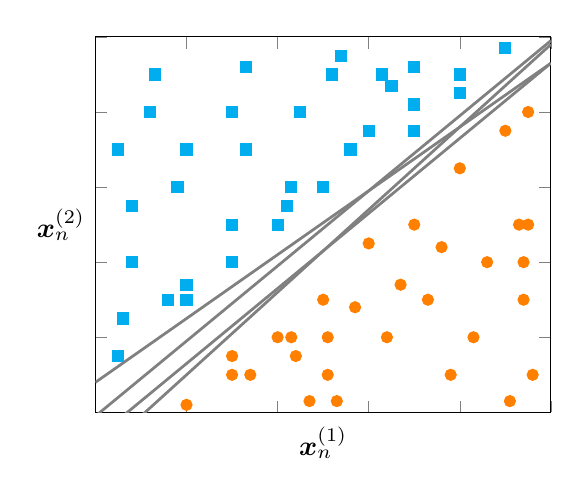
\begin{tikzpicture}
            \begin{axis}[ 
                width= 2.9in,
                height= 2.5in,
                xlabel=$\bm{x}_n^{(1)}$,
                ylabel={$\bm{x}_n^{(2)}$},
                yticklabels={,,},
                xticklabels={,,},
                xmin=0,
                xmax=10,
                ymin=0,
                ymax=10,
                every axis x label/.style={
                    at={(axis description cs:0.5,-0.15)},
                    anchor=south
                },
                every axis y label/.style={
                    at={(axis description cs:-0.15,.5)},
                    anchor=west
                },
            ]
            \addplot+[only marks,mark=square*,mark options={scale=1, color=cyan}] coordinates {
                (0.5,1.5) (0.6,2.5) (0.8,5.5) (0.8,4) (0.5,7)
                (1.2,8) (1.3,9) (1.6,3) (1.8,6) 
                (2,3) (2,3.4) (2,7) 
                (3,4) (3,8) (3,5) (3.3,7) (3.3,9.2)
                (4,5) (4.2,5.5) (4.3,6) (4.5,8) 
                (5,6) (5.2,9) (5.4,9.5) (5.6,7) 
                (6,7.5) (6.3,9) (6.5,8.7) 
                (7,7.5) (7,9.2) (7,8.2) 
                (8,8.5) (8,9)
                (9,9.7)
            };
            
            \addplot+[only marks,mark=*,mark options={scale=1, color=orange}] coordinates {
                (2,0.2)
                (3,1.5) (3,1) (3.4,1) 
                (4,2) (4.7,0.3) (4.4,1.5) (4.3,2) 
                (5,3) (5.1,1) (5.1,2) (5.3,0.3) (5.7,2.8) 
                (6,4.5) (6.4,2) (6.7,3.4) 
                (7,5) (7.3,3) (7.8,1) (7.6,4.4) 
                (8,6.5) (8.3,2) (8.6,4) 
                (9,7.5) (9.1,0.3) (9.3,5) (9.4,3) (9.4,4)
                (9.5,8) (9.5,5) (9.6,1) 
            };
            
            \addplot [
                domain=0:10, 
                samples=100, 
                color=gray,
                style={line width=1pt}
            ]
            {x - 0.7};
            
            \addplot [
                domain=0:10, 
                samples=100, 
                color=gray,
                style={line width=1pt}
            ]
            {1.1*x - 1.2};
            
            \addplot [
                domain=0:10, 
                samples=100, 
                color=gray,
                style={line width=1pt}
            ]
            {0.85*x + 0.8};
            
            \addplot [
                domain=0:10, 
                samples=100, 
                color=gray,
                style={line width=1pt}
            ]
            {1*x - 0.1};
          \end{axis}
        \end{tikzpicture}
        \captionsetup{labelfont={bf}, textfont=it, width=.8\linewidth}
        \caption{Candidate linear classifiers. There are more multiple hyperplanes that classify the training data without error.}\label{fig:candidate seperating hyperplanes}
    \end{center}
\end{figure}

Our derivation of the SVM algorithm is yet to be complete: consider, for instance, a linearly separable training data set and the hyperplane that solves the classification problem. As illustrated in Figure \ref{fig:candidate seperating hyperplanes}, there are often infinite many candidate linear classifiers which will classify the training data without incurring any training error or ``bias"; hence, we need to further develop our algorithm to systematically find a unique linear classifier. We elaborate on how we choose this unique ideal separator in Section \ref{sec:the margin}.

Even more concerning model's inability to train on a non-linearly separable data set. Since linearly separable training data is rarely available in the real world, we need to tweak our model by allowing examples to fall on the wrong side of the hyperplane thereby allowing the model to incur training error as explored in Section \ref{sec:soft margin}.

\subsubsection{Maximum Margin Derivation}\label{sec:the margin}
To find the ideal linear classifier we look for a hyperplane with the largest buffer between it and the nearest example. This buffer is called the margin and is a prevailing concept in not just this paper but in the entire field of machine learning\footnote{Refer to \textit{Learning with Kernels} \citep{scholkopf2002learning} to explore how concepts like the margin and empirical risk minimization extend into other machine learning algorithms}. Imagine a two-way street running between two blocks of houses. The center line which separates the two lanes represents the hyperplane. This center line is painted where the distance between it and the houses on either side is maximized and equivalent. This is so the lanes on either side are at their widest which is ideal for traffic. Similarly, we seek to find the candidate hyperplane with the largest margin in between it and nearest training data. Before rigorously solving for this hyperplane, there is a technical point we need to first consider: the scale to measure distance from the hyperplane. We cannot use the scale of the data because we can change the units of measurement of any feature in $\bm{x}_n$ and the scale would change thereby changing its distance to the hyperplane. The solution is to instead base the scale on the equation for the hyperplane itself.

Consider an example $\bm{x}_n \in \mathbb{R}^D$ and the  hyperplane $\langle \bm{w}, \bm{x}_n \rangle + b = 0$. Suppose $\bm{x}_n$ lies on the positive side of the hyperplane and let $r > 0$ be the distance between $\bm{x}_n$ and the hyperplane. Recall the Orthogonal Decomposition Theorem \citep{lay2016linear} states the distance between $\bm{y} \in \mathbb{R}^D$  and a subspace $U$ of $\mathbb{R}^D$ is the distance from $\bm{y}$ to the orthogonal projection $\pi_U(\bm{y}_i)$ of $\bm{y}$ onto $U$. With this intuition we can find the distance $r$ with the orthogonal projection of $\bm{x}_n$ onto the hyperplane:

\begin{definition}[Orthogonal decomposition for affine subspaces]
    Let $L = \bm{w} + H$ be an affine subspace of $\mathbb{R}^D$. The vector $\bm{x} \in \mathbb{R}^D$ can be written uniquely as
    \begin{subequations}
        \begin{align}
            \bm{x} & = \pi_L(\bm{x}) + \bm{z} \\
            & = \pi_H(\bm{x} - \bm{w}) + \bm{w} + \bm{z}
        \end{align}
    \end{subequations}
    where $\pi_L(\bm{x})$ is the orthogonal projection of $\bm{x}$ onto the affine subspace $L$.
\end{definition}
The projection $\pi_L(\bm{x})$ is identical to the orthogonal projection of $\bm{x} - \bm{w}$ onto $H$ translated back onto $L$ by adding $\bm{w}$. More importantly, the closest vector to $\bm{x}$ on $L$ is still the orthogonal projection $\pi_L(\bm{x})$:
\begin{subequations}
    \begin{align}
        \textrm{dist}(\bm{x}, L) & = \norm{\bm{x} - \pi_L(\bm{x})} = \norm{\bm{x} - (\pi_H(\bm{x} - \bm{w}) + \bm{w})} \\
        & = \textrm{dist}(\bm{x} - \bm{w}, \pi_H(\bm{x} - \bm{w})) \\
        & = \textrm{dist}(\bm{x} - \bm{w}, H)
    \end{align}
\end{subequations}

Recall we are trying to find the distance $r > 0$ from an example $\bm{x}_n$ to the hyperplane. We do this with the orthogonal projection $\bm{\hat{x}}_n$ of $\bm{x}_n$ onto the hyperplane. We know $\bm{x}_n - \bm{\hat{x}}_n$ is orthogonal to the hyperplane and hence from Proposition \ref{prop:w is normal} a scaling of $\bm{w}$. By normalizing $\bm{w}$ then scaling it by the distance $r$ we obtain
\begin{equation}\label{eq:orthogonal decomposition on hyperplane}
    \bm{x}_n = \bm{\hat{x}}_n + r \frac{\bm{w}}{\norm{\bm{w}}}.
\end{equation}
We suppose $r$ is our margin, i.e., $\bm{x}_n$ is the nearest example to the hyperplane; therefore, other examples must be at least a distance $r$ from the hyperplane in the positive or negative direction. This constraint combined with \eqref{eq:correct side constraint} gives the inequality
\begin{equation} \label{eq:r margin constraint}
    y_n (\langle \bm{w}, \bm{x}_n \rangle + b) \geq r.
\end{equation}
We also suppose $\bm{w}$ is of unit length using the Euclidean norm, i.e., $\norm{\bm{w}} = \sqrt{\bm{w}^\intercal \bm{w}} = 1$. Recall the goal is to maximize the margin $r$ under this new constraint such that each example is distanced $r$ or greater from the hyperplane given $r>0$ and $\norm{\bm{w}}=1$. We translate this objective and constraints into the constrained optimization problem
\begin{subequations}\label{eq:optimization problem 1}
    \begin{align}
        \max_{\bm{w}, b, r} \quad & r \\
        \textrm{subject to} \quad & y_n (\langle \bm{w}, \bm{x}_n \rangle + b) \geq r, \\
        & \norm{\bm{w}}=1,\label{eq:parameter vector is unit} \\
        & r > 0  \\
        & \textrm{for all} \quad n = 1, \dots, N.
    \end{align}
\end{subequations}
Fortunately, this turns out to be a convex optimization problem for which there exists many competent programming libraries. When handed off to a package, a program will solve for the values of $\bm{w}, b, r$ such that margin is maximized and the data is lying on the correct side of the hyperplane.

At last we have formalized a rudimentary SVM algorithm able to be performed by a computer. In order to develop this algorithm further, we pause to consider the traditional approach at deriving the margin.

\subsubsection{Tradition Margin Derivation}
We obtained a constrained optimization problem \eqref{eq:optimization problem 1} which solves for the ideal hyperplane that classifies linearly separable data. Our derivation in Section \ref{sec:the margin} is not the conventional and often more confusing derivation. In our first derivation we assumed the parameter vector $\bm{w}$ is of unit length, i.e., $\norm{\bm{w}}=1$. Traditionally, however, we choose a scale for our data rather than choosing the length of our parameter vector. We choose a scale such that the predictor $y_n(\langle \bm{w}, \bm{x}_n \rangle + b)$ has the value $1$ at the closest example to the hyperplane $\bm{x}_a$. Geometrically, we can understand this by imagining two parallel hyperplanes $\langle \bm{w}, \bm{x}_n \rangle + b = -1$ and $\langle \bm{w}, \bm{x}_n \rangle + b = +1$ acting as boundaries which the data must lie outside of. Note that this implies there should be no data in the buffer between boundaries and the hyperplane. By definition since the orthogonal projection $\bm{\hat{x}}_a$ is on the hyperplane, $\langle \bm{w}, \bm{\hat{x}}_a \rangle + b = 0$. This with \eqref{eq:orthogonal decomposition on hyperplane} and the bilinearity of the inner product gives
\begin{subequations}
    \begin{align}
        \langle \bm{w}, \bm{x}_a - r \frac{\bm{w}}{\norm{\bm{w}}} \rangle + b & = 0 \\
        \langle \bm{w}, \bm{x}_a \rangle + b - r \frac{\langle \bm{w}, \bm{w} \rangle}{\norm{\bm{w}}} & = 0 \\
        \langle \bm{w}, \bm{x}_a \rangle + b & = r \norm{\bm{w}}.
    \end{align}
\end{subequations}
By our assumption $\langle \bm{w}, \bm{x}_a \rangle + b = 1$, we observe the first term in the last line is $1$. Therefore we obtain the crucial observation
\begin{equation}
    r = \frac{1}{\norm{\bm{w}}}.
\end{equation}
We combine this with Equation 8 and get the condition
\begin{equation}
    y_n (\langle \bm{w}, \bm{x}_n \rangle + b) \geq 1.
\end{equation}
This brings us to a constrained optimization problem similar to (9),
\begin{equation}
    \begin{split}
        \max_{\bm{w}, b} \quad & \frac{1}{\norm{\bm{w}}} \\
        \textrm{subject to} \quad & y_n (\langle \bm{w}, \bm{x}_n \rangle + b) \geq r \\
        & \textrm{for all} \quad n = 1, \dots, N.
    \end{split}
\end{equation}
Maximizing $\frac{1}{\norm{\bm{w}}}$ is observably the same objective as minimizing $\norm{\bm{w}}$. Conventionally $\norm{\bm{w}}$ is squared and multiplied by the constant $\frac{1}{2}$ as to allow for tidier calculations when computing the gradient and using Lagrange multipliers. Note that our objective does not change. With these alterations we arrive at the traditional algorithm for the \textit{hard margin SVM}.
\begin{equation}
    \begin{split}
        \min_{\bm{w}, b} \quad & \frac{1}{2} \norm{\bm{w}}^2 \\
        \textrm{subject to} \quad & y_n (\langle \bm{w}, \bm{x}_n \rangle + b) \geq r \\
        & \textrm{for all} \quad n = 1, \dots, N.
    \end{split}
\end{equation}

\begin{theorem}\label{theorem}
    Maximizing the margin r under constraints as in \eqref{eq:optimization problem 1} is equivalent to scaling the data such that the margin is 1:
    \begin{subequations}\label{eq:optimization problem 2}
        \begin{align}
            \min_{\bm{w}, b} \quad & \frac{1}{2} \norm{\bm{w}}^2 \\
            \textnormal{subject to} \quad & y_n (\langle \bm{w}, \bm{x}_n \rangle + b) \geq r \\
            & \textnormal{for all} \quad n = 1, \dots, N.
        \end{align}
    \end{subequations}
\end{theorem}
\begin{proof}
    Consider \eqref{eq:optimization problem 1}. Let $\bm{w'} = \lambda\bm{w}$ for some scalar $\lambda \in \mathbb{R}$. Since $\norm{\bm{w}} = 1$ from \eqref{eq:parameter vector is unit},
    \begin{equation}
        \bm{w} = \frac{\bm{w'}}{\lambda} =  \frac{\bm{w'}}{\norm{\bm{w'}}}.
    \end{equation}
    We reparametrize to obtain
    \begin{subequations}
        \begin{align}
            \max_{\bm{w'}, b, r} \quad & r \label{eq:listen to ghosttown by kanye}\\
            \textrm{subject to} \quad & y_n (\langle \frac{\bm{w'}}{\norm{\bm{w'}}}, \bm{x}_n \rangle + b) \geq r, \\
            & r > 0 \label{eq:positive margin} \\
            & \textrm{for all} \quad n = 1, \dots, N.
        \end{align}
    \end{subequations}
    Let $\bm{w''} = \frac{\bm{w'}}{\norm{\bm{w'}}r}$ and $b'' = \frac{b}{r}$. The constraint \eqref{eq:positive margin} states the distance $r$ is positive. Therefore, we divide both sides of \eqref{eq:listen to ghosttown by kanye} by $r$ and reparametrize to obtain
    \begin{subequations}
        \begin{align}
            \max_{\bm{w''}, b, r} \quad & r \\
            \textrm{subject to} \quad & y_n (\langle \bm{w''}, \bm{x}_n \rangle + b'') \geq 1, \\
            & r > 0  \\
            & \textrm{for all} \quad n = 1, \dots, N.
        \end{align}
    \end{subequations}
    % \begin{lemma} $r = \frac{1}{\bm{w''}}$ \end{lemma}
    % \begin{proof}
    %     Suppose $\bm{\hat{x}}_a$ is the closest example to the  Let $\bm{\hat{x}}_n$ be the orthogonal projection of $\bm{x}_n$ onto the hyperplane \eqref{eq:svm hyperplane}. Since $\bm{\hat{x}}_n$ is on the hyperplane,
    %     \begin{equation}
    %         \langle \bm{w}, \bm{\hat{x}}_n \rangle = 0.
    %     \end{equation}
    %     Substituting \label{eq:orthogonal decomposition on hyperplane} and exploiting a property of inner product gives
    %     \begin{subequations}
    %         \begin{align}
    %             \langle \bm{w}, \bm{x}_n - r \frac{\bm{w''}}{\norm{\bm{w''}}} \rangle = 0. \\
    %             \textrm{subject to} \quad & y_n (\langle \bm{w''}, \bm{x}_n \rangle + b'') \geq 1, \\
    %             & r > 0  \\
    %             & \textrm{for all} \quad n = 1, \dots, N.
    %         \end{align}
    %     \end{subequations}
    % \end{proof}
    Rearranging $\bm{w''} = \frac{\bm{w'}}{\norm{\bm{w'}}r}$ for $r$ gives
    \begin{equation}
        \norm{\bm{w''}} = \norm{\frac{\bm{w'}}{\norm{\bm{w'}}r}} = \frac{1}{r} \norm{\frac{\bm{w'}}{\norm{\bm{w'}}}} = \frac{1}{r}.
    \end{equation}
    The objective does not change if we chose to maximize $r^2$ instead of $r$ since the square is strictly monotonic for $r>0$. By substituting we obtain
    \begin{subequations}
        \begin{align}
            \max_{\bm{w''}, b} \quad & \frac{1}{\norm{\bm{w''}}} \\
            \textrm{subject to} \quad & y_n (\langle \bm{w''}, \bm{x}_n \rangle + b'') \geq 1, \\
            & \textrm{for all} \quad n = 1, \dots, N.
        \end{align}
    \end{subequations}
    Maximizing $\frac{1}{\norm{\bm{w''}}}$ is observably equivalent to minimizing $\frac{1}{2}\norm{\bm{w''}}$ so we choose this to be the objective, thereby giving \eqref{eq:optimization problem 2}.
\end{proof}
Theorem \ref{theorem} gives us the optimization problem of the hard margin SVM \eqref{eq:optimization problem 2}. The ``hard margin" comes from how examples are not allowed to be within the margin or on the wrong side of the hyperplane. With our new algorithm let's perform a test on real world data.

\subsubsection{Hard Margin SVM and the Iris Data Set}
\begin{figure}
    \begin{center}
        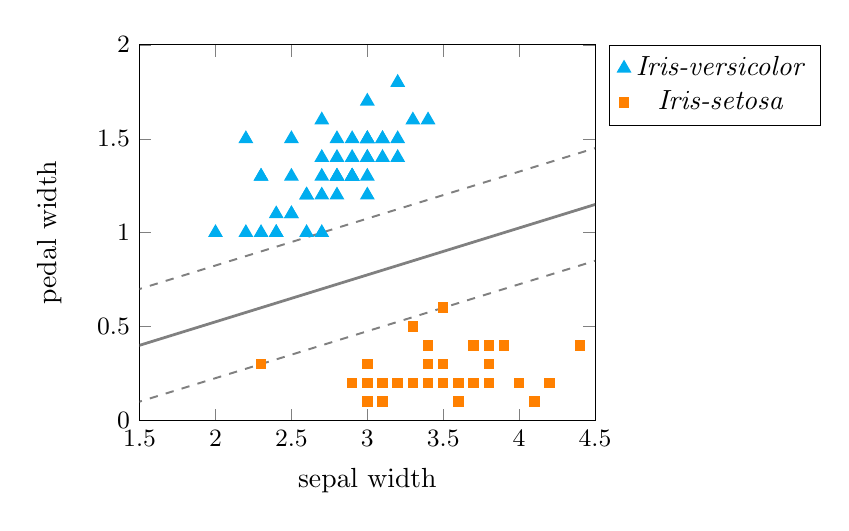
\begin{tikzpicture}
            \begin{axis}[
                width=2.9in,
                height=2.5in,
                xlabel={sepal width},
                ylabel={pedal width},
                xtick={1.5, 2.0, 2.5, 3.0, 3.5, 4.0, 4.5},
                ticklabel style = {font=\small},
                xmin=1.5,
                xmax=4.5,
                ymin=0,
                ymax=2.0,
                every axis x label/.style={
                    at={(axis description cs:0.5, -0.22)},
                    anchor=south
                },
                every axis y label/.style={
                    at={(axis description cs: -0.15, 0.5)},
                    anchor=south,
                    rotate=90
                },
                legend pos=outer north east
            ]
            \addplot+[only marks,mark=triangle*,mark options={scale=1.35, color=cyan}] coordinates {
                (3.2, 1.4) (3.2, 1.5) (3.1, 1.5) (2.3, 1.3) (2.8, 1.5) (2.8, 1.3) (3.3, 1.6) (2.4, 1) (2.9, 1.3) (2.7, 1.4) (2, 1) (3, 1.5) (2.2, 1) (2.9, 1.4) (2.9, 1.3) (3.1, 1.4) (3, 1.5) (2.7, 1) (2.2, 1.5) (2.5, 1.1) (3.2, 1.8) (2.8, 1.3) (2.5, 1.5) (2.8, 1.2) (2.9, 1.3) (3, 1.4) (2.8, 1.4) (3, 1.7) (2.9, 1.5) (2.6, 1) (2.4, 1.1) (2.4, 1) (2.7, 1.2) (2.7, 1.6) (3, 1.5) (3.4, 1.6) (3.1, 1.5) (2.3, 1.3) (3, 1.3) (2.5, 1.3) (2.6, 1.2) (3, 1.4) (2.6, 1.2) (2.3, 1) (2.7, 1.3) (3, 1.2) (2.9, 1.3) (2.9, 1.3) (2.5, 1.1) (2.8, 1.3)
            };
            \addlegendentry{\textit{Iris-versicolor}}
            
            \addplot+[only marks,mark=square*,mark options={scale=0.85, color=orange}] coordinates {
                (3.5, .2) (3, .2) (3.2, .2) (3.1, .2) (3.6, .2) (3.9, .4) (3.4, .3) (3.4, .2) (2.9, .2) (3.1, .1) (3.7, .2) (3.4, .2) (3, .1) (3, .1) (4, .2) (4.4, .4) (3.9, .4) (3.5, .3) (3.8, .3) (3.8, .3) (3.4, .2) (3.7, .4) (3.6, .2) (3.3, .5) (3.4, .2) (3, .2) (3.4, .4) (3.5, .2) (3.4, .2) (3.2, .2) (3.1, .2) (3.4, .4) (4.1, .1) (4.2, .2) (3.1, .2) (3.2, .2) (3.5, .2) (3.6, .1) (3, .2) (3.4, .2) (3.5, .3) (2.3, .3) (3.2, .2) (3.5, .6) (3.8, .4) (3, .3) (3.8, .2) (3.2, .2) (3.7, .2) (3.3, .2)
            };
            \addlegendentry{\textit{Iris-setosa}}
            
            \addplot [
                domain=0:10, 
                samples=100, 
                color=gray,
                style={line width=0.7pt,
                dashed}
            ]
            {0.25*x + 0.325};
            
            \addplot [
                domain=0:10, 
                samples=100, 
                color=gray,
                style={line width=1pt}
            ]
            {0.25*x + 0.025};
            
            \addplot [
                domain=0:10, 
                samples=100, 
                color=gray,
                style={line width=0.7pt,
                dashed}
            ]
            {0.25*x - 0.275};
          \end{axis}
        \end{tikzpicture}
        \captionsetup{labelfont={bf}, textfont=it, width=.8\linewidth}
        \caption{Fisher's Iris Data Set classified with a hard margin SVM. Two classes of iris flowers and two features.}
        \label{fig:Fisher's Iris data set example 1}
    \end{center}
\end{figure}

Take the example of the \textit{Fisher's Iris data set} \citep{irisdataset}, an exceptionally popular data set in the data science community. It consists of measurements of 150 iris flowers across three species: \textit{Iris-setosa}, \textit{Iris-versicolor}, and \textit{Iris-virginica}. For each individual flower 4 measurements were made: pedal width, pedal length, sepal width, sepal length. Since the hard margin SVM algorithm we have designed only performs binary classification on linearly separable data, we chose two of the three classes (\textit{Iris-setosa}, \textit{Iris-versicolor}) and two of the four features (sepal width, pedal width).

If one were to draw a linear classifier by hand, there would be many to choose from. However, the ``best" linear classifier (as we defined in Section \ref{sec:the margin}) coincides with the linear classifier returned by our SVM. As evident in Figure \ref{fig:Fisher's Iris data set example 1}, the SVM returned a linear separator with the largest possible margin. Flowers of the same species fall on the same side of the hyperplane, thus incurring no training error and therefore no bias. We already have an extremely competent algorithm able to optimally linearly separable binary classification data. Unfortunately, until now we have only considered linearly separable data. In most cases the data will not be linearly separable as in Figure\ref{fig:Fisher's Iris data set example 1}. To adapt our algorithm, we reexamine the margin.

\subsection{The Soft Margin SVM}\label{sec:soft margin}

\begin{figure}
    \centering
    \begin{subfigure}{0.3\textwidth}
        \begin{center}
            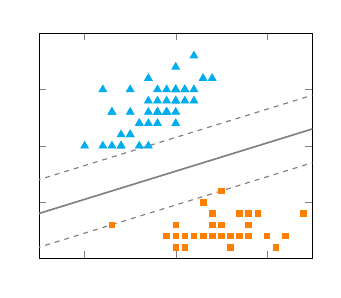
\begin{tikzpicture}[scale=0.60]
                \begin{axis}[
                    width=2.9in,
                    height=2.5in,
                    yticklabels={,,},
                    xticklabels={,,},
                    xmin=1.5,
                    xmax=4.5,
                    ymin=0,
                    ymax=2.0,
                    every axis x label/.style={
                        at={(axis description cs:0.5, -0.22)},
                        anchor=south
                    },
                    every axis y label/.style={
                        at={(axis description cs: -0.15, 0.5)},
                        anchor=south,
                        rotate=90
                    }
                ]
                \addplot+[only marks,mark=triangle*,mark options={scale=1.35, color=cyan}] coordinates {
                    (3.2, 1.4) (3.2, 1.5) (3.1, 1.5) (2.3, 1.3) (2.8, 1.5) (2.8, 1.3) (3.3, 1.6) (2.4, 1) (2.9, 1.3) (2.7, 1.4) (2, 1) (3, 1.5) (2.2, 1) (2.9, 1.4) (2.9, 1.3) (3.1, 1.4) (3, 1.5) (2.7, 1) (2.2, 1.5) (2.5, 1.1) (3.2, 1.8) (2.8, 1.3) (2.5, 1.5) (2.8, 1.2) (2.9, 1.3) (3, 1.4) (2.8, 1.4) (3, 1.7) (2.9, 1.5) (2.6, 1) (2.4, 1.1) (2.4, 1) (2.7, 1.2) (2.7, 1.6) (3, 1.5) (3.4, 1.6) (3.1, 1.5) (2.3, 1.3) (3, 1.3) (2.5, 1.3) (2.6, 1.2) (3, 1.4) (2.6, 1.2) (2.3, 1) (2.7, 1.3) (3, 1.2) (2.9, 1.3) (2.9, 1.3) (2.5, 1.1) (2.8, 1.3)
                };

                \addplot+[only marks,mark=square*,mark options={scale=0.85, color=orange}] coordinates {
                    (3.5, .2) (3, .2) (3.2, .2) (3.1, .2) (3.6, .2) (3.9, .4) (3.4, .3) (3.4, .2) (2.9, .2) (3.1, .1) (3.7, .2) (3.4, .2) (3, .1) (3, .1) (4, .2) (4.4, .4) (3.9, .4) (3.5, .3) (3.8, .3) (3.8, .3) (3.4, .2) (3.7, .4) (3.6, .2) (3.3, .5) (3.4, .2) (3, .2) (3.4, .4) (3.5, .2) (3.4, .2) (3.2, .2) (3.1, .2) (3.4, .4) (4.1, .1) (4.2, .2) (3.1, .2) (3.2, .2) (3.5, .2) (3.6, .1) (3, .2) (3.4, .2) (3.5, .3) (2.3, .3) (3.2, .2) (3.5, .6) (3.8, .4) (3, .3) (3.8, .2) (3.2, .2) (3.7, .2) (3.3, .2)
                };

                \addplot [
                    domain=0:10, 
                    samples=100, 
                    color=gray,
                    style={line width=0.7pt,
                    dashed}
                ]
                {0.25*x + 0.325};
                
                \addplot [
                    domain=0:10, 
                    samples=100, 
                    color=gray,
                    style={line width=1pt}
                ]
                {0.25*x + 0.025};
                
                \addplot [
                    domain=0:10, 
                    samples=100, 
                    color=gray,
                    style={line width=0.7pt,
                    dashed}
                ]
                {0.25*x - 0.275};
              \end{axis}
            \end{tikzpicture}
            \captionsetup{labelfont={bf}, textfont=it, width=.9\linewidth}
            \caption{$C=10^2$; slack minimization prioritized significantly over margin maximization.}
            \label{fig:iris data soft margin 1}
        \end{center}
    \end{subfigure}
    \begin{subfigure}{0.3\textwidth}
        \begin{center}
            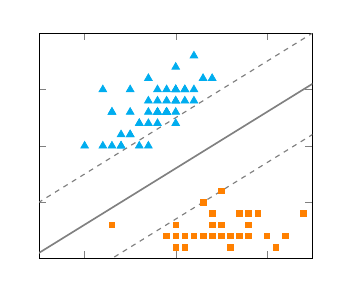
\begin{tikzpicture}[scale=0.60]
                \begin{axis}[
                    width=2.9in,
                    height=2.5in,
                    yticklabels={,,},
                    xticklabels={,,},
                    xmin=1.5,
                    xmax=4.5,
                    ymin=0,
                    ymax=2.0,
                    every axis x label/.style={
                        at={(axis description cs:0.5, -0.22)},
                        anchor=south
                    },
                    every axis y label/.style={
                        at={(axis description cs: -0.15, 0.5)},
                        anchor=south,
                        rotate=90
                    },
                ]
                \addplot+[only marks,mark=triangle*,mark options={scale=1.35, color=cyan}] coordinates {
                    (3.2, 1.4) (3.2, 1.5) (3.1, 1.5) (2.3, 1.3) (2.8, 1.5) (2.8, 1.3) (3.3, 1.6) (2.4, 1) (2.9, 1.3) (2.7, 1.4) (2, 1) (3, 1.5) (2.2, 1) (2.9, 1.4) (2.9, 1.3) (3.1, 1.4) (3, 1.5) (2.7, 1) (2.2, 1.5) (2.5, 1.1) (3.2, 1.8) (2.8, 1.3) (2.5, 1.5) (2.8, 1.2) (2.9, 1.3) (3, 1.4) (2.8, 1.4) (3, 1.7) (2.9, 1.5) (2.6, 1) (2.4, 1.1) (2.4, 1) (2.7, 1.2) (2.7, 1.6) (3, 1.5) (3.4, 1.6) (3.1, 1.5) (2.3, 1.3) (3, 1.3) (2.5, 1.3) (2.6, 1.2) (3, 1.4) (2.6, 1.2) (2.3, 1) (2.7, 1.3) (3, 1.2) (2.9, 1.3) (2.9, 1.3) (2.5, 1.1) (2.8, 1.3)
                };

                \addplot+[only marks,mark=square*,mark options={scale=0.85, color=orange}] coordinates {
                    (3.5, .2) (3, .2) (3.2, .2) (3.1, .2) (3.6, .2) (3.9, .4) (3.4, .3) (3.4, .2) (2.9, .2) (3.1, .1) (3.7, .2) (3.4, .2) (3, .1) (3, .1) (4, .2) (4.4, .4) (3.9, .4) (3.5, .3) (3.8, .3) (3.8, .3) (3.4, .2) (3.7, .4) (3.6, .2) (3.3, .5) (3.4, .2) (3, .2) (3.5, .2) (3.4, .2) (3.2, .2) (3.1, .2) (3.4, .4) (4.1, .1) (4.2, .2) (3.1, .2) (3.2, .2) (3.5, .2) (3.6, .1) (3, .2) (3.4, .2) (3.5, .3) (2.3, .3) (3.2, .2) (3.5, .6) (3.8, .4) (3, .3) (3.8, .2) (3.2, .2) (3.7, .2) (3.3, .2)
                };

                \addplot [
                    domain=0:10, 
                    samples=100, 
                    color=gray,
                    style={line width=0.7pt,
                    dashed}
                ]
                {0.50*x - 0.25};
                
                \addplot [
                    domain=0:10, 
                    samples=100, 
                    color=gray,
                    style={line width=1pt}
                ]
                {0.50*x - 0.7};
                
                \addplot [
                    domain=0:10, 
                    samples=100, 
                    color=gray,
                    style={line width=0.7pt,
                    dashed}
                ]
                {0.50*x - 1.15};
              \end{axis}
            \end{tikzpicture}
            \captionsetup{labelfont={bf}, textfont=it, width=.9\linewidth}
            \caption{$C=10^0$; slack minimization and margin maximization prioritized evenly.}
            \label{fig:iris data soft margin 2}
        \end{center}
    \end{subfigure}
    \begin{subfigure}{0.3\textwidth}
        \begin{center}
            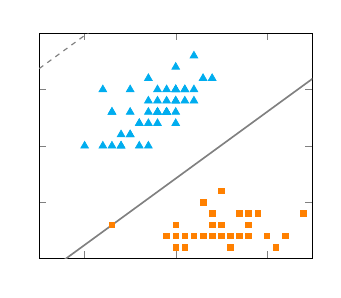
\begin{tikzpicture}[scale=0.60]
                \begin{axis}[
                    width=2.9in,
                    height=2.5in,
                    yticklabels={,,},
                    xticklabels={,,},
                    xmin=1.5,
                    xmax=4.5,
                    ymin=0,
                    ymax=2.0,
                    every axis x label/.style={
                        at={(axis description cs:0.5, -0.22)},
                        anchor=south
                    },
                    every axis y label/.style={
                        at={(axis description cs: -0.15, 0.5)},
                        anchor=south,
                        rotate=90
                    },
                ]
                \addplot+[only marks,mark=triangle*,mark options={scale=1.35, color=cyan}] coordinates {
                    (3.2, 1.4) (3.2, 1.5) (3.1, 1.5) (2.3, 1.3) (2.8, 1.5) (2.8, 1.3) (3.3, 1.6) (2.4, 1) (2.9, 1.3) (2.7, 1.4) (2, 1) (3, 1.5) (2.2, 1) (2.9, 1.4) (2.9, 1.3) (3.1, 1.4) (3, 1.5) (2.7, 1) (2.2, 1.5) (2.5, 1.1) (3.2, 1.8) (2.8, 1.3) (2.5, 1.5) (2.8, 1.2) (2.9, 1.3) (3, 1.4) (2.8, 1.4) (3, 1.7) (2.9, 1.5) (2.6, 1) (2.4, 1.1) (2.4, 1) (2.7, 1.2) (2.7, 1.6) (3, 1.5) (3.4, 1.6) (3.1, 1.5) (2.3, 1.3) (3, 1.3) (2.5, 1.3) (2.6, 1.2) (3, 1.4) (2.6, 1.2) (2.3, 1) (2.7, 1.3) (3, 1.2) (2.9, 1.3) (2.9, 1.3) (2.5, 1.1) (2.8, 1.3)
                };

                \addplot+[only marks,mark=square*,mark options={scale=0.85, color=orange}] coordinates {
                    (3.5, .2) (3, .2) (3.2, .2) (3.1, .2) (3.6, .2) (3.9, .4) (3.4, .3) (3.4, .2) (2.9, .2) (3.1, .1) (3.7, .2) (3.4, .2) (3, .1) (3, .1) (4, .2) (4.4, .4) (3.9, .4) (3.5, .3) (3.8, .3) (3.8, .3) (3.4, .2) (3.7, .4) (3.6, .2) (3.3, .5) (3.4, .2) (3, .2) (3.4, .4) (3.5, .2) (3.4, .2) (3.2, .2) (3.1, .2) (3.4, .4) (4.1, .1) (4.2, .2) (3.1, .2) (3.2, .2) (3.5, .2) (3.6, .1) (3, .2) (3.4, .2) (3.5, .3) (2.3, .3) (3.2, .2) (3.5, .6) (3.8, .4) (3, .3) (3.8, .2) (3.2, .2) (3.7, .2) (3.3, .2)
                };

                \addplot [
                    domain=0:10, 
                    samples=100, 
                    color=gray,
                    style={line width=0.7pt,
                    dashed}
                ]
                {0.59*x + 0.8};
                
                \addplot [
                    domain=0:10, 
                    samples=100, 
                    color=gray,
                    style={line width=1pt}
                ]
                {0.59*x - 1.06};
              \end{axis}
            \end{tikzpicture}
            \captionsetup{labelfont={bf}, textfont=it, width=.9\linewidth}
            \caption{$C=10^{-2}$; margin maximization prioritized significantly over slack minimization.}
            \label{fig:iris data soft margin 3}
        \end{center}
    \end{subfigure}
    \captionsetup{labelfont={bf}, textfont=it, width=.8\linewidth}
    \caption{Fisher's Iris Data Set classified using a soft margin SVM at varying values for the regularization parameter $C$.}
    \label{fig:iris data soft margin}
\end{figure}

\subsubsection{Slack and Regularization}
To adapt the algorithm to be able to train on non-linearly separable data sets, we need to allow some examples to fall within the margin region or even on the wrong side of the hyperplane. We do this by giving each example-label pair $(\bm{x}_n, y_n)$ a ``slack variable" $\xi_n > 0$. When training the model, this slack allows examples to be correctly classified while falling on the wrong side of the margin. We still want to minimize the number of examples which fall on the wrong side of the margin, therefore we aim to minimize the total slack across all examples-label pairs. Combining this additional objective and constraints we obtain the optimization problem
\begin{subequations}\label{eq:optimization problem 3}
    \begin{align}
        \min_{\bm{w}, b, \xi} \quad & \frac{1}{2}  \norm{\bm{w}}^2 + C\sum_{n=1}^{N} \xi_n \\
        \textrm{subject to} \quad & y_n (\langle \bm{w}, \bm{x}_n \rangle + b) \geq r - \xi_n \\
        & \xi_n \geq 0 \\
        & \textrm{for all} \quad n = 1, \dots, N.
    \end{align}
\end{subequations}

The SVM with this optimization problem is called the soft margin SVM since examples can cross the margin. The constant $C>0$ is referred to as the ``regularization parameter". The regularization parameter trades off total amount of slack for maximizing the margin. A larger value of $C$ gives a higher priority to minimize slack in the objective: the SVM will emphasize minimizing how many examples fall on the incorrect side of the margin over maximizing the margin. In the real world, the value of $C$ is optimized with cross-validation, a process which estimates the model parameters that produce the lowest variance.

\subsubsection{Soft Margin SVM and the Iris Data Set}

\begin{figure}
    \centering
    \begin{tabular}{lll}\toprule
    $C$       & bias (\%)  & variance (\%) \\ \midrule
    $10^{-2}$ & $23.72$              & $28.4$ \\
    $10^{-1}$ & $7.88$               & $18.4$ \\
    $10^{0}$  & $1.12$               & $16.8$ \\
    $10^{1}$  & $0.16$               & $19.4$ \\
    $10^{2}$  & $0.08$               & $19.4$ \\
    $10^{3}$  & $0.08$               & $19.4$ \\ \bottomrule
    \end{tabular}
    \captionsetup{labelfont={bf}, textfont=it, width=.8\linewidth}
    \caption{Training and test error on different values for the regularization parameter $C$.}
    \label{fig:regularization parameter}
\end{figure}

Again consider the same \textit{Fisher's Iris data set} as before\footnote{The axis and legend of Figure \ref{fig:iris data soft margin} are consistent with Figure \ref{fig:Fisher's Iris data set example 1}.}. We used a hard margin SVM to find the linear classifier in Figure \ref{fig:Fisher's Iris data set example 1}. The hard margin SVM is equivalent to the soft margin SVM with infinitely expensive slack, i.e., a soft margin SVM where the regularization parameter is infinitely large. The table in Figure \ref{fig:regularization parameter} demonstrates how the training error approaches $0$\% as the regularization parameter grows larger. Different values of the regularization parameter is illustrated in Figure \ref{fig:iris data soft margin}. As we can see, with a lower value of the regularization parameter as in Figure \ref{fig:iris data soft margin 3} means maximizing the margin even if training error rises. The table reveals that the model is optimal, i.e., has the least variance, when $C=10^0$ (see Figure \ref{fig:iris data soft margin 2}). By simply introducing the ability for examples to cross the margin, we have derived an algorithm which empirically reduces testing error. This allows us to more confidently employ this algorithm in real world situations.

\newpage

\section{Conclusion}

\subsection{Furthur Reading}
The soft margin SVM derived in this paper is widely employed in all fields of science including biology (seen with the \textit{Fisher's Iris data set} examples), medicine (in patient diagnoses), and in aerospace engineering for object detection. To read more on the applications of the concepts talk about in the scope of this paper, refer to \textit{Support Vector Machine Applications} \citep{ma2014support} which takes a particular emphasis on the SVM in medicine. A natural continuation of this paper is to learn about the Dual SVM; \textit{An Introduction to Support Vector Machines: And Other Kernel-Based Learning  Methods} \citep{cristianini2014introduction} explores the dual form of our SVM algorithm which optimizes performance on more complex data sets sometimes upwards of a million dimensions. A slower and more thorough iteration of this paper's derivations can be found in \textit{Support Vector Machines} \citep{steinwart2008support}.

\subsection{Bibliography}

\bibliographystyle{plain}
\bibliography{references}

\end{document}
